%%%%%%%%%%%%%%%%%%%%%%%%%%%%%%%%%%%%%%%%%%%%%%%%%%%%%%%%%%%%%%%%%%%%%%%%%%%%%%%%
\section{Why Workflow Managers?}
{   
	\usebackgroundtemplate{
		\vbox to \paperheight{\vfil\hbox to \paperwidth{\hfil
\includegraphics[height=.7\paperheight]{humor/DALLE_LEGO-scientist-thinking}\hfil}\vfil}
	}
	\frame{
		\frametitle{Why use Workflow Managers?}
		\begin{mdframed}[tikzsetting={draw=white,fill=white,fill opacity=0.8,
				line width=0pt},backgroundcolor=none,leftmargin=0,
			rightmargin=150,innertopmargin=4pt,roundcorner=10pt]
			\tableofcontents[currentsection,sections={1-4},hideothersubsections]
		\end{mdframed}
		\vspace{12mm}\hfill{\tiny \lhref{https://zenodo.org/records/11147887}{from Ewa Bres \& Christian Bittner}}
	}
}

%%%%%%%%%%%%%%%%%%%%%%%%%%%%%%%%%%%%%%%%%%%%%%%%%%%%%%%%%%%%%%%%%%%%%%%%%%%%%%%%
\begin{frame}
  \frametitle{What is this about?}
   \begin{question}[Questions]
   	 \begin{itemize}
        \item Let them learn the batch system! Really?
        \item What is the benefit of a workflow system for admins?
        \item What distinguishes a workflow system from a ``pipeline''?
     \end{itemize}
   \end{question}
   \begin{docs}[Objectives]
   	  \begin{enumerate}
         \item Introducing workflow engines (particularly \Snakemake)!
      \end{enumerate}
   \end{docs}
\end{frame}  

%%%%%%%%%%%%%%%%%%%%%%%%%%%%%%%%%%%%%%%%%%%%%%%%%%%%%%%%%%%%%%%%%%%%%%%%%%%%%%%%
\begin{frame}
	\frametitle{Data Analysis}
	\centering
	\begin{onlyenv}<1| handout:0>
		\begin{tikzpicture}
			\path[use as bounding box] (feat/admin_talk0.7,0) rectangle (12,8);
			\node[inner sep=0pt] (analysis_1) at (5,5.5)
			{\includegraphics[width=0.7\textwidth]{Snakemake/analysis_1.png}};   
			\node at (7, 3.5) %[below=-0.4cm of analysis_1, xshift=2.7cm] at (current page.center)
			{\includegraphics[width=0.45\textwidth]{Snakemake/phd_left.png}};
			\node at (6, 1) {\begin{minipage}{0.75\textwidth}\footnotesize
					Idea from the official \lhref{https://slides.com/johanneskoester/snakemake-tutorial}{\Snakemake} course (with permission), image from \lhref{https://phdcomics.com/comics.php}{PhD comics}.
				\end{minipage}
			};
		\end{tikzpicture}    
	\end{onlyenv}
	
	\begin{onlyenv}<2| handout:1>
		\begin{tikzpicture}
			\path[use as bounding box] (0.7,0) rectangle (12,8);
			\node[inner sep=0pt] (analysis_full) at (5,5.5)
			{\includegraphics[width=0.7\textwidth]{Snakemake/analysis_full.png}};   
			\node at (7,3.5) % [below=-0.4cm of analysis_full, xshift=2.7cm]
			{\includegraphics[width=0.45\textwidth]{Snakemake/phd_full.png}};
			\node at (6, 1) {\begin{minipage}{0.75\textwidth}\footnotesize
					Idea from the official \lhref{https://slides.com/johanneskoester/snakemake-tutorial}{\Snakemake} course (with permission), image from \lhref{https://phdcomics.com/comics.php}{PhD comics}.
				\end{minipage}
			};
		\end{tikzpicture}
	\end{onlyenv}
\end{frame}

%%%%%%%%%%%%%%%%%%%%%%%%%%%%%%%%%%%%%%%%%%%%%%%%%%%%%%%%%%%%%%%%%%%%%%%%%%%%%%%%
\begin{frame}
	\frametitle{Let them learn SLURM!}
	\centering
	
\includegraphics[width=0.9\textwidth]{humor/Leonardo_Depict_former_French_Queen_Marie_Antoinett.jpg}
\end{frame}	

%%%%%%%%%%%%%%%%%%%%%%%%%%%%%%%%%%%%%%%%%%%%%%%%%%%%%%%%%%%%%%%%%%%%%%%%%%%%%%%%
\begin{frame}
	\frametitle{Constituents of a Data Analysis Workflow $\ldots$}
	\ldots (almost) regardless of research topic!
	\centering
	\vfill
	\smartdiagram[sequence diagram]{
		{QC},
		{processing [multiple steps]},
		{summary statistics},
		{report / plots}}
    \vfill
    \pause
    \begin{hint}
    	Not all steps are "HPC-worthy"! E.g. plotting / visualization, moving data, etc.
    \end{hint}
\end{frame}

%%%%%%%%%%%%%%%%%%%%%%%%%%%%%%%%%%%%%%%%%%%%%%%%%%%%%%%%%%%%%%%%%%%%%%%%%%%%%%%%
\begin{frame}[t]
 \frametitle{Meet: The DAG!}
 \begin{docs}
 	\emph{Every} data analysis workflow can be expressed as a \bf{D}irected \bf{A}cyclic \bf{G}raph - a DAG.
 \end{docs}
 \vspace{4em}
 \pause
 \begin{columns}
 	\begin{column}{0.4\textwidth}
 		\begin{minipage}[t]{\textwidth}
 			\centering
 			The rulegraph:\newline
 			\includegraphics[width=0.4\textwidth]{workflows/complete_workflow.png}
 		\end{minipage}
 		
 	\end{column}
    \begin{column}{0.6\textwidth}
    	\pause
    	\begin{minipage}[t]{\textwidth}
    	   \centering
    	   The full DAG - for every sample:\newline
    	   \includegraphics[width=0.9\textwidth]{workflows/book.png}
        \end{minipage}
    	
    	
    \end{column}
 \end{columns}
 \vfill
\end{frame}

%%%%%%%%%%%%%%%%%%%%%%%%%%%%%%%%%%%%%%%%%%%%%%%%%%%%%%%%%%%%%%%%%%%%%%%%%%%%%%%%
\begin{frame}[t]
	\frametitle{Interlude: An Example}
	\vspace{-3em}
	\begin{columns}[t]
		\begin{column}{0.6\textwidth}
			\begin{hint}[Background]
				This example is one coded in Bash with SLURM dependencies \emph{and} \Snakemake. This is its DAG:
				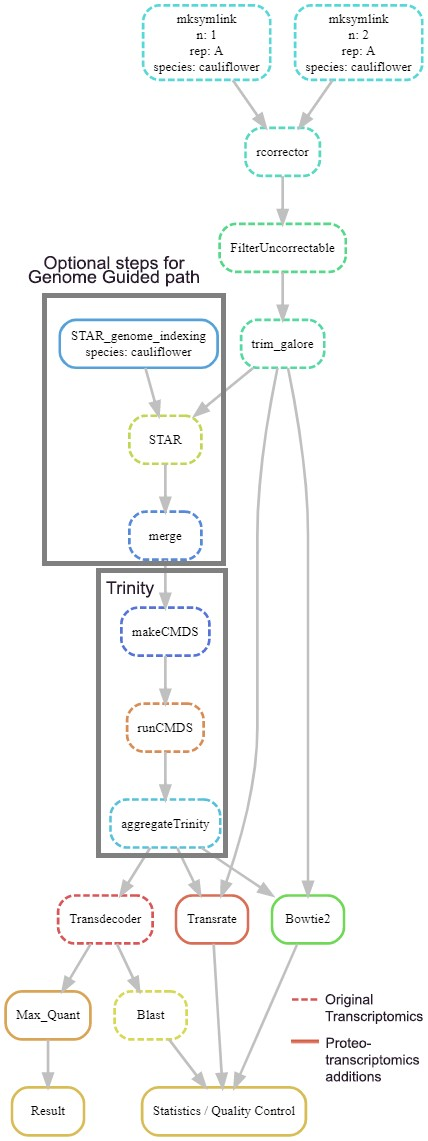
\includegraphics[width=0.25\textwidth]{workflows/proteo_transcriptomics.jpeg} 
			\end{hint}
		\end{column}
	    \begin{column}{0.4\textwidth}
	    	\begin{question}
	    		What does it take to code this using Bash and SLURM commands, only?
	    	\end{question}
    	    \pause
    	    \begin{warning}
    	    	%Fasten your seat-belts!
    	    	Now would follow a long section of fast displayed slides with bash code. We will skip this to save time.
    	    \end{warning}
	    \end{column}
	\end{columns}
    \vfill
\end{frame}

%%%%%%%%%%%%%%%%%%%%%%%%%%%%%%%%%%%%%%%%%%%%%%%%%%%%%%%%%%%%%%%%%%%%%%%%%%%%%%%%% 
%\begin{frame}[fragile]
%	\frametitle{Asynchronous Execution using the Batch System}
%	\begin{onlyenv}<1>{An Proteomics-Workflows will serve as an example (Bash Files + wildly cloned internet stuff):
%			
%			\begin{lstlisting}[language=Bash, style=Shell, basicstyle=\TINY]  
%#!/bin/bash
%
%#SBATCH -N 1
%##SBATCH -c 1
%#SBATCH -A jgu-multiomics
%#SBATCH -p nodeshort                   # may consider running on a bigmem node for large dataset
%##SBATCH -e fastqc_%A.err            # File to which STDERR will be written
%#SBATCH -o fastqc_%A.out           # File to which STDOUT will be written
%#SBATCH -J fastqc_%A               # Job name
%#SBATCH --mem-per-cpu=8G
%##SBATCH --mem=50G                # Memory requested (mega default units)
%##SBATCH --ramdisk=150G
%#SBATCH --time=05:00:00              # Runtime in D-HH:MM:SS
%
%module purge   
%set -x
%
%REFDIR=$1
%SPECIES=$2
%REP=$3
%OUTPUT_FOLDER=fastqc_results/${SPECIES}/rep_${REP}
%mkdir -p ${OUTPUT_FOLDER}
%
%
%
%for i in ${REFDIR}/Sample_imb_butter_*_${SPECIES}_${REP}_*.fastq.gz
%do
%    fastqc -o ./${OUTPUT_FOLDER}/ $i
%done
%	\end{lstlisting}}\end{onlyenv}
%	
%	\begin{onlyenv}<2>\begin{lstlisting}[language=Bash, style=Shell, basicstyle=\TINY]
%#!/bin/bash
%
%#SBATCH -N 1
%#SBATCH -c 32 #64
%#SBATCH -A m2_imb-pga
%#SBATCH -p bigmem #parallel
%#SBATCH -C skylake
%#SBATCH -e correctr_%A.err            # File to which STDERR will be written
%#SBATCH -o correctr_%A.out           # File to which STDOUT will be written
%#SBATCH -J READcorrect_%A               # Job name
%#SBATCH --mem=354000 #350G              # 50G originally Memory requested (mega default units)
%##SBATCH --ramdisk=350G  # 150G originally
%#SBATCH --time=05:00:00              # Runtime in D-HH:MM:SS
%
%# LOAD RELEVANT MODULES FOR STEP 2
%module purge
%#module load bio/Rcorrector/1.0.4-foss-2019a
%module load bio/Jellyfish/2.2.6
%module load lang/Perl/5.26.1-foss-2017a
%module load lang/Python/2.7.13-foss-2017a
%set -x
%
%# RESERVE RAMDISK SPACE
%JOBDIR=/localscratch/$SLURM_JOB_ID
%RAMDISK=$JOBDIR
%mkdir -p $RAMDISK
%
%#SET VARIABLES
%#REFDIR=/gpfs/fs2/project/jgu-multiomics/Michal/EvoReg/RNAseq_rawdata/imb_butter_2014_04_EvoReg_RNASeq
%#REFDIR=$1
%#SPECIES=$2
%#REP=$3
%OUTPUT_FOLDER=trimmed_reads/${SPECIES}/rep_${REP}
%mkdir -p ${OUTPUT_FOLDER}
%
%
%#COPY FASTQ.GZ FILES TO RAMDISK
%file_list=( $(find $REF_DIR -name ${REP}*.gz ) )
%for fname in "${file_list[@]}"; do
%    #cp -rL ${fname} ${RAMDISK}/.
%    STEM=$(basename "${fname}" .gz)
%    gunzip -c ${fname} > ${RAMDISK}/${STEM}
%done
%#R1_file=( $( find ${RAMDISK} -regextype sed -regex '.*/*[\-\_\.]\(R1\|read1\|Read1\|READ1\)[\-\_\.]*(fastq\|fq)' ) )
%#R1_file=( $( find ${RAMDISK} -regex '.*/*[\-\_\.]\(R1\|read1\|Read1\|READ1\)[\-\_\.]*(fastq\|fq)' ) )
%R1_file=( $( find ${RAMDISK} -type f | egrep "*[._-](read1|Read1|r1|R1)*[._-](fq|fastq)" ) )
%echo $R1_file
%#R2_file=( $( find ${RAMDISK} -regextype sed -regex '.*/*[\-\_\.]\(R2\|read2\|Read2\|READ2\)[\-\_\.]*(fastq\|fq)' ) )
%R2_file=( $( find ${RAMDISK} -type f | egrep "*[._-](read2|Read2|r1|R2)*[._-](fq|fastq)" ) )
%#R2_file=( $( find ${RAMDISK} -regex '.*/*[\-\_\.]\(R2\|read2\|Read2\|READ2\)[\-\_\.]*(fastq\|fq)' ) )
%echo $R2_file
%
%# FIRST STEP: REMOVE K-MERS
%${RAMDISK}/*[-_.]@(R1|read1|Read1|READ1)[-_.]*fastq ${RAMDISK}/*[-_.]@(R2|read2|Read2|READ2)[-_.]*fastq
%
%perl programs_ProTrans/rcorrector/run_rcorrector.pl -od ${RAMDISK}/ -t $SLURM_CPUS_PER_TASK -p ${R1_file} ${R2_file}
%wait
%module purge
%module load lang/Python/2.7.13-foss-2017a
%python programs_ProTrans/FilterUncorrectabledPEfastq.py -1 ${RAMDISK}/*R1.cor.fq  -2 ${RAMDISK}/*R2.cor.fq  -o $RAMDISK/fixed 2>&1 > ${RAMDISK}/rmunfixable.out
%wait
%rm ${R1_file}
%rm ${R2_file}
%
%# SECOND STEP: REMOVE ADAPTERS AND LOW QUALITY REGIONS
%module purge
%module load bio/FastQC/0.11.9-Java-11
%module load bio/cutadapt/2.10-GCCcore-8.3.0-Python-3.7.4
%module load bio/Trim_Galore/0.6.5-GCCcore-8.3.0-Java-11-Python-3.7.4
%
%trim_galore --paired --retain_unpaired --phred33 --output_dir $RAMDISK --length 36 -q 5 --stringency 1 -e 0.1 $RAMDISK/fixed*R1.cor.fq $RAMDISK/fixed*R2.cor.fq
%
%trimmed_reads --length 36 -q 5 --stringency 1 -e 0.1 ./fixed*R1.cor.fq ./fixed*R2.cor.fq
%wait
%cp ${RAMDISK}/fixed_*.cor_val_*.fq $OUTPUT_FOLDER
%	\end{lstlisting}\end{onlyenv}
%	\begin{onlyenv}<3>\begin{lstlisting}[language=Bash, style=Shell, basicstyle=\TINY]
%#!/bin/bash 
%
%#SBATCH -N 1
%#SBATCH -c 12
%#SBATCH -A m2_imb-pga
%#SBATCH -p smp                   # may consider running on a bigmem node for large dataset
%#SBATCH -e build_genome_%A.err            # File to which STDERR will be written
%#SBATCH -o build_genome_%A.out           # File to which STDOUT will be written
%#SBATCH -J build_genome_%A               # Job name
%#SBATCH --mem=100G                 # Memory requested (mega default units)
%#SBATCH --time=00:30:00              # Runtime in D-HH:MM:SS
%#SBATCH --mail-type=ALL              # Type of email notification- BEGIN,END,FAIL,ALL
%#SBATCH --mail-user=m.levin@imb.de # Email to send notifications to
%#SBATCH --ramdisk=100G
%
%module load bio/STAR/2.5.3a-foss-2017a
%
%STAR_FOLDER=${GENOME_FILE%.*.*}_STAR_index
%
%mkdir -p $STAR_FOLDER
%
%
%JOBDIR=/localscratch/$SLURM_JOB_ID
%RAMDISK=$JOBDIR/ramdisk
%
%#gunzip $GENOME_FILE
%zcat $GENOME_FILE > $RAMDISK/temp.fa
%#GENOME_FILE_uz="$(ls $GENOME_FILE/*.fa)"
%
%STAR --runMode genomeGenerate --outTmpDir $RAMDISK/tmp --genomeDir $STAR_FOLDER --genomeFastaFiles $RAMDISK/temp.fa --runThreadN $SLURM_CPUS_PER_TASK --limitGenomeGenerateRAM 60000000000 --outFileNamePrefix $STAR_FOLDER
%	\end{lstlisting}\end{onlyenv}
%	\begin{onlyenv}<4>\begin{lstlisting}[language=Bash, style=Shell, basicstyle=\TINY]
%#!/bin/bash
%
%#SBATCH -p parallel
%#SBATCH -C skylake
%#SBATCH -N 1
%#SBATCH -c 16
%#SBATCH -A m2_imb-pga
%##SBATCH -e MAP4Trinity_%A.err            # File to which STDERR will be written
%#SBATCH -o MAP4Trinity_%A.out           # File to which STDOUT will be written
%#SBATCH -J MAP4Trinity_%A               # Job name
%#SBATCH --mem=177000 #350G                # Memory requested (mega default units)
%#SBATCH --ramdisk=450G
%#SBATCH --time=03:00:00 #05:00:00              # Runtime in D-HH:MM:SS
%#SBATCH --mail-type=ALL              # Type of email notification- BEGIN,END,FAIL,ALL
%#SBATCH --mail-user=m.levin@imb.de # Email to send notifications to
%
%module load bio/STAR/2.5.3a-foss-2017a
%
%STAR_FOLDER=${STAR_FOLDER_LOC}
%OUTPUT_FOLDER=${WORK_DIR}/mapped/${SPECIES}/
%
%mkdir -p $OUTPUT_FOLDER
%mkdir -p ${OUTPUT_FOLDER}/log_files
%set -x
%
%JOBDIR=/localscratch/$SLURM_JOB_ID
%RAMDISK=$JOBDIR/ramdisk
%mkdir -p $RAMDISK
%
%REFDIR=trimmed_reads/${SPECIES}/rep_${REP}
%
%cp $REFDIR/*R1.cor_val_1.fq $RAMDISK/R1.fq
%#gzip $RAMDISK/$species'_R1.fq' 
%cp $REFDIR/*R2.cor_val_2.fq $RAMDISK/R2.fq
%#gzip $RAMDISK/$species'_R2.fq'
%
%wait
%
%STAR --runThreadN $SLURM_CPUS_PER_TASK --genomeDir $STAR_FOLDER --outSAMtype BAM SortedByCoordinate --outFileNamePrefix $RAMDISK/${SPECIES}_rep_${REP}_ --alignIntronMax $MAX_INTRON_SIZE --limitBAMsortRAM 6000463617 --outFilterMultimapNmax 1 --outFilterScoreMin 20 --readFilesIn $RAMDISK/R1.fq $RAMDISK/R2.fq
%
%
%wait
%
%cp $RAMDISK/${SPECIES}_rep_${REP}_Aligned.sortedByCoord.out.bam $OUTPUT_FOLDER
%cp $RAMDISK/${SPECIES}_rep_${REP}_Log* $OUTPUT_FOLDER/log_files
%cp $RAMDISK/${SPECIES}_rep_${REP}_SJ.out.tab $OUTPUT_FOLDER/log_files
%	\end{lstlisting}\end{onlyenv}
%	\begin{onlyenv}<5>\begin{lstlisting}[language=Bash, style=Shell, basicstyle=\TINY]
%#!/bin/bash
%
%#SBATCH -N 1
%#SBATCH -p bigmem
%#SBATCH -C skylake
%#SBATCH -A m2_imb-pga
%#SBATCH -c 64
%#SBATCH --ramdisk=400G
%#SBATCH -e trinity_normalization_%A.err            # File to which STDERR will be written
%#SBATCH -o trinity_normalization_%A.out           # File to which STDOUT will be written
%#SBATCH -J trinity_normalization_%A               # Job name
%#SBATCH --mem=354000 #350G                 # Memory requested (mega default units)
%##SBATCH --mem=100G                 # Memory requested (mega default units)
%#SBATCH --time=1-20:00:00 #07:00:00 #1-20:00:00              # Runtime in D-HH:MM:SS
%#SBATCH --mail-type=ALL              # Type of email notification- BEGIN,END,FAIL,ALL
%#SBATCH --mail-user=m.levin@imb.de # Email to send notifications to
%
%#module load bio/SAMtools/1.9-foss-2018a
%module purge
%module load bio/Trinity/2.8.4-foss-2018a
%#module load lang/Python/3.6.4-foss-2017a
%#module load bio/Jellyfish/2.2.6-foss-2017a
%#module load bio/SAMtools/1.5-foss-2017a
%#module load bio/Bowtie2/2.3.2-foss-2017a
%module load bio/Salmon/0.13.1-foss-2018a
%
%OUTPUT_FOLDER=trinity_GF_split_allbamcomb/$SPECIES
%mkdir -p $OUTPUT_FOLDER/trinity
%
%### START THE TRINITY ASSEMBLY ONLY IF THE RESPECTIVE trinity_GG.cmds FILE DOES NOT YET EXIST
%if [ ! -f $OUTPUT_FOLDER/trinity/recursive_trinity.cmds ]; then
%    echo "recursive_trinity.cmds for species "$SPECIES" does not yet exist. Starting job to create"
%		
%	JOBDIR=/localscratch/$SLURM_JOB_ID
%	RAMDISK=$JOBDIR/ramdisk
%	#RAMDISK=$JOBDIR
%	mkdir -p $RAMDISK
%	mkdir -p $RAMDISK/trinity
%	
%	REFDIR=${WORK_DIR}/trimmed_reads/${SPECIES}
%	
%	cat $(find ${REFDIR}/ -type f -name '*.R1.*')  > ${RAMDISK}/R1.fq
%	cat $(find ${REFDIR}/ -type f -name '*.R2.*')  > ${RAMDISK}/R2.fq 
%	wait
%	
%	#Trinity --genome_guided_bam $RAMDISK/*.bam --genome_guided_max_intron $INTRON_MAX --max_memory $((SLURM_MEM_PER_NODE / 1024))G --CPU $SLURM_CPUS_PER_TASK --SS_lib_type FR --output $OUTPUT_FOLDER/trinity
%
%	#Trinity --genome_guided_bam $RAMDISK/*.bam --genome_guided_max_intron $INTRON_MAX --max_memory $((SLURM_SPANK_JOB_RAMDISK / 1024))G --CPU $SLURM_CPUS_PER_TASK --SS_lib_type FR --full_cleanup --verbose --output $RAMDISK/trinity
%	
%	Trinity --seqType fq --SS_lib_type RF --max_memory 50G --min_kmer_cov $min_kmer_cov --CPU $SLURM_CPUS_PER_TASK --left $RAMDISK/R1.fq --right $RAMDISK/R2.fq --output $OUTPUT_FOLDER/trinity --full_cleanup --verbose --no_distributed_trinity_exec
%		
%		
%		
%	# --max_memory $((SLURM_MEM_PER_NODE / 1024))G 
%else
%	echo "Trinity.fasta for species "$SPECIES" already exists - nothing to do here!"
%fi
%	\end{lstlisting}\end{onlyenv}
%	\begin{onlyenv}<6>\begin{lstlisting}[language=Bash, style=Shell, basicstyle=\TINY]
%#!/bin/bash
%
%#SBATCH -A m2_imb-pga 
%#SBATCH -n 1
%#SBATCH --job-name=trinity_arrayJob
%##SBATCH --output=trinity_arrayJob_%A_%a.out # redirecting stdout
%##SBATCH --error=trinity_arrayJob_%A_%a.err  # redirecting stderr
%##SBATCH --array=1-712
%##SBATCH --array=5
%#SBATCH --time=15:00:00 #15:00:00
%#SBATCH --partition=smp #parallel 
%#SBATCH --ntasks=1        # number of tasks per array job
%#SBATCH --mem-per-cpu=20000 #4000  #20000
%##SBATCH --cpus-per-task=1 
%#SBATCH --mail-type=ALL              # Type of email notification- BEGIN,END,FAIL,ALL
%#SBATCH --mail-user=m.levin@imb.de # Email to send notifications to
%##SBATCH --mem-per-cpu=8000
%module load bio/Trinity/2.8.4-foss-2018a
%module load bio/Salmon/0.13.1-foss-2018a
%
%CMD_FILE=recursive_trinity.cmds
%CMD_NO=$(wc -l recursive_trinity.cmds | awk '{print $1}')
%echo "Number of commands in recursive.cmds file is:"
%echo $CMD_NO
%echo "This is array No.:"
%echo $SLURM_ARRAY_TASK_ID
%((CHUNKSIZE=(CMD_NO/SLURM_ARRAY_TASK_COUNT)+1))
%((TOTALREST=500*CHUNKSIZE))
%((REDUCED_JOBS=TOTALREST-CMD_NO))
%((NUM_JOBS=500-((REDUCED_JOBS/CHUNKSIZE)+1)))
%arrayID=$SLURM_ARRAY_TASK_ID
%			
%if [ "$arrayID" -lt "$NUM_JOBS" ]; then
%	indexes=`seq $(((((arrayID - 1) * CHUNKSIZE) + 1))) $(((((arrayID - 1) * CHUNKSIZE) + CHUNKSIZE)))`
%	echo "Processing command lines: "
%	echo $(((((arrayID - 1) * CHUNKSIZE) + 1)))
%	echo "to"
%	echo $(((((arrayID - 1) * CHUNKSIZE) + CHUNKSIZE)))
%	for i in $indexes ; do
%		echo "################################"
%		echo "Processing cmds line:"
%		echo $i
%		echo "################################"
%		bash -c "$(head -n $i ${CMD_FILE} | tail -n 1)"
%	done
%elif [ "$arrayID" -eq "$NUM_JOBS" ]; then
%	indexes=`seq $(((((arrayID - 1) * CHUNKSIZE) + 1))) $CMD_NO`
%	echo "This is the last array and processes the remaining commands till end of cmd file"   
%	echo "Processing command lines: "
%	echo $(((((arrayID - 1) * CHUNKSIZE) + 1)))
%	echo "to"
%	echo $CMD_NO
%    for i in $indexes ; do
%		echo "################################"
%		echo "Processing cmds line:"
%		echo $i
%		echo "################################"
%		bash -c "$(head -n $i ${CMD_FILE} | tail -n 1)"
%	done
%else
%	#indexes=`seq 1 1`
%	#echo "This is just a placeholder array re-processing first command"
%	echo "This is an empty script"
%fi
%	\end{lstlisting}\end{onlyenv}
%	\begin{onlyenv}<7>\begin{lstlisting}[language=Bash, style=Shell, basicstyle=\TINY]
%#!/bin/bash
%
%#SBATCH -N 1
%#SBATCH -c 1
%#SBATCH -A m2_imb-pga
%#SBATCH -p smp                   # may consider running on a bigmem node for large dataset
%#SBATCH -e ph_%A.err            # File to which STDERR will be written
%#SBATCH -o ph_%A.out           # File to which STDOUT will be written
%#SBATCH -J ph_%A               # Job name
%#SBATCH --mem=50M    #500M             # Memory requested (mega default units)
%#SBATCH --time=03:00:00              # Runtime in D-HH:MM:SS
%#SBATCH --mail-type=ALL              # Type of email notification- BEGIN,END,FAIL,ALL
%#SBATCH --mail-user=m.levin@imb.de # Email to send notifications to
%
%module load bio/Trinity/2.8.4-foss-2018a
%
%REF_DIR=${WORK_DIR}/trinity_GF_split_allbamcomb/${SPECIES}/trinity
%
%#find ${REF_DIR}/read_partitions/  -name '*inity.fasta'  | /gpfs/fs1/cluster/easybuild/nehalem/software/bio/Trinity/2.8.4-foss-2017a/trinityrnaseq-Trinity-v2.8.4/util/support_scripts/partitioned_trinity_aggregator.pl TRINITY_DN > ${REF_DIR}/Trinity-GF.fasta
%
%find ${REF_DIR}/read_partitions/  -name '*inity.fasta'  | /cluster/easybuild/broadwell/software/bio/Trinity/2.8.4-foss-2018a/trinityrnaseq-Trinity-v2.8.4/util/support_scripts/partitioned_trinity_aggregator.pl --token_prefix TRINITY_DN --output_prefix ${REF_DIR}/Trinity-GF
%	\end{lstlisting}\end{onlyenv}
%	\begin{onlyenv}<8>\begin{lstlisting}[language=Bash, style=Shell, basicstyle=\TINY]
%#!/bin/bash
%
%#SBATCH -N 1
%#SBATCH -c 1
%#SBATCH -A m2_imb-pga
%#SBATCH -p smp
%##SBATCH -e ph_%A.err            # File to which STDERR will be written
%##SBATCH -o ph_%A.out           # File to which STDOUT will be written
%##SBATCH -J ph_%A               # Job name
%##SBATCH --mem=1K                # Memory requested (mega default units)
%#SBATCH --time=00:30:00              # Runtime in D-HH:MM:SS
%##SBATCH --mail-type=ALL              # Type of email notification- BEGIN,END,FAIL,ALL
%##SBATCH --mail-user=m.levin@imb.de # Email to send notifications to
%
%echo 'Moving final file!'
%
%REF_DIR=${WORK_DIR}/trinity_GF_split_allbamcomb/${SPECIES}/trinity
%FINAL_DIR=${WORK_DIR}/Trinity_GF_assemblies
%
%cp ${REF_DIR}/Trinity-GF.fasta  ${FINAL_DIR}/Trinity-GF_${SPECIES}_mincov${min_kmer_cov}.fasta
%wait
%mkdir -p ${WORK_DIR}/trinity_GF_split_allbamcomb/${SPECIES}/blanktemp
%rsync -a --delete ${WORK_DIR}/trinity_GF_split_allbamcomb/${SPECIES}/blanktemp/ ${WORK_DIR}/trinity_GF_split_allbamcomb/${SPECIES}/
%wait
%	\end{lstlisting}\end{onlyenv}
%	\begin{onlyenv}<9>\begin{lstlisting}[language=Bash, style=Shell, basicstyle=\TINY]
%#!/bin/bash
%
%#SBATCH -N 1
%#SBATCH -p bigmem
%#SBATCH -C skylake
%#SBATCH -A m2_imb-pga
%#SBATCH -c 64
%#SBATCH --ramdisk=400G
%#SBATCH -e trinity_normalization_%A.err            # File to which STDERR will be written
%#SBATCH -o trinity_normalization_%A.out           # File to which STDOUT will be written
%#SBATCH -J trinity_normalization_%A               # Job name
%#SBATCH --mem=354000 #500G                 # Memory requested (mega default units)
%#SBATCH --time=1-20:00:00 #10:00:00 #1-20:00:00              # Runtime in D-HH:MM:SS
%#SBATCH --mail-type=ALL              # Type of email notification- BEGIN,END,FAIL,ALL
%#SBATCH --mail-user=m.levin@imb.de # Email to send notifications to
%
%set -x
%
%#module load bio/SAMtools/1.9-foss-2018a
%module purge
%module load bio/Trinity/2.8.4-foss-2018a
%#module load lang/Python/3.6.4-foss-2017a
%#module load bio/Jellyfish/2.2.6-foss-2017a
%#module load bio/SAMtools/1.5-foss-2017a
%#module load bio/Bowtie2/2.3.2-foss-2017a
%module load bio/Salmon/0.13.1-foss-2018a
%
%OUTPUT_FOLDER=trinity_GG_split_allbamcomb/$SPECIES
%mkdir -p $OUTPUT_FOLDER/trinity
%
%### START THE TRINITY ASSEMBLY ONLY IF THE RESPECTIVE trinity_GG.cmds FILE DOES NOT YET EXIST
%if [ ! -f $OUTPUT_FOLDER/trinity/trinity_GG.cmds ]; then
%    echo "trinity_GG.cmds for species "$SPECIES" does not yet exist. Starting job to create"
%
%    JOBDIR=/localscratch/$SLURM_JOB_ID
%    RAMDISK=$JOBDIR/ramdisk
%    mkdir -p $RAMDISK
%    mkdir -p $RAMDISK/trinity
%
%    REFDIR=${WORK_DIR}/mapped/${SPECIES}
%    #REL_FILE=zebrafinch_rep_C_Aligned.sortedByCoord.out.bam
%    ### use the biggest bam file available for the species 
%    FILES_2_COMB=$(find ${REFDIR}/ -name '*_Aligned.sortedByCoord.out.bam' | xargs echo) 
%    #REL_FILE=$(du -cks $REFDIR/*.bam | sort -n -r | awk '{print $2}' | head -n2 | tail -n1 | cut -d'/' -f11)
%    samtools merge $RAMDISK/merged.bam $FILES_2_COMB
%
%    wait
%
%    Trinity --genome_guided_bam $RAMDISK/merged.bam --genome_guided_max_intron $MAX_INTRON_SIZE --genome_guided_min_coverage $genome_guided_min_coverage --max_memory $((SLURM_MEM_PER_NODE / 1024))G --CPU $SLURM_CPUS_PER_TASK --SS_lib_type FR --full_cleanup --verbose --no_distributed_trinity_exec --output $OUTPUT_FOLDER/trinity
%			
%			
%	else
%		echo "Trinity-GG.fasta for species "$SPECIES" already exists - nothing to do here!"
%fi
%	\end{lstlisting}\end{onlyenv}
%	
%	\begin{onlyenv}<10>\begin{lstlisting}[language=Bash, style=Shell, basicstyle=\TINY]
%#!/bin/bash
%
%#SBATCH -A m2_imb-pga 
%#SBATCH -n 1
%#SBATCH --job-name=trinity_arrayJob
%##SBATCH --output=trinity_arrayJob_%A_%a.out # redirecting stdout
%##SBATCH --error=trinity_arrayJob_%A_%a.err  # redirecting stderr
%#SBATCH --array=1-712
%##SBATCH --array=5
%#SBATCH --time=15:00:00 #15:00:00
%#SBATCH --partition=smp
%#SBATCH --ntasks=1        # number of tasks per array job
%#SBATCH --mem-per-cpu=20000 #4000 #20000
%##SBATCH --cpus-per-task=1 
%#SBATCH --mail-type=ALL              #
%Type of email notification- BEGIN,END,FAIL,ALL
%#SBATCH --mail-user=m.levin@imb.de # Email to send notifications to
%
%module load bio/Trinity/2.8.4-foss-2018a
%module load bio/Salmon/0.13.1-foss-2018a
%
%CMD_FILE=trinity_GG.cmds
%CMD_NO=$(wc -l trinity_GG.cmds | awk '{print $1}')
%
%echo "Number of commands in recursive.cmds file is:"
%echo $CMD_NO
%echo "This is array No.:"
%echo $SLURM_ARRAY_TASK_ID
%((CHUNKSIZE=(CMD_NO/SLURM_ARRAY_TASK_COUNT)+1))
%((TOTALREST=500*CHUNKSIZE))
%((REDUCED_JOBS=TOTALREST-CMD_NO))
%((NUM_JOBS=500-((REDUCED_JOBS/CHUNKSIZE)+1)))
%arrayID=$SLURM_ARRAY_TASK_ID
%			
%if [ "$arrayID" -lt "$NUM_JOBS" ]; then
%	indexes=`seq $(((((arrayID - 1) * CHUNKSIZE) + 1))) $(((((arrayID - 1) * CHUNKSIZE) + CHUNKSIZE)))`
%	echo "Processing command lines: "
%	echo $(((((arrayID - 1) * CHUNKSIZE) + 1)))
%	echo "to"
%	echo $(((((arrayID - 1) * CHUNKSIZE) + CHUNKSIZE)))
%	for i in $indexes ; do
%		echo "################################"
%		echo "Processing cmds line:"
%		echo $i
%		echo "################################"
%		bash -c "$(head -n $i ${CMD_FILE} | tail -n 1)"
%	done
%elif [ "$arrayID" -eq "$NUM_JOBS" ]; then
%	indexes=`seq $(((((arrayID - 1) * CHUNKSIZE) + 1))) $CMD_NO`
%	echo "This is the last array and processes the remaining commands till end of cmd file"   
%	echo "Processing command lines: "
%	echo $(((((arrayID - 1) * CHUNKSIZE) + 1)))
%	echo "to"
%	echo $CMD_NO
%	for i in $indexes ; do
%		echo "################################"
%		echo "Processing cmds line:"
%		echo $i
%		echo "################################"
%		bash -c "$(head -n $i ${CMD_FILE} | tail -n 1)"
%	done
%else
%	#indexes=`seq 1 1`
%	#echo "This is just a placeholder array re-processing first command"
%	echo "This is an empty script"
%fi
%	\end{lstlisting}\end{onlyenv}
%	\begin{onlyenv}<11>\begin{lstlisting}[language=Bash, style=Shell, basicstyle=\TINY]
%#!/bin/bash
%
%#SBATCH -N 1
%#SBATCH -c 1
%#SBATCH -A m2_imb-pga
%#SBATCH -p smp
%#SBATCH -e ph_%A.err            # File to which STDERR will be written
%#SBATCH -o ph_%A.out           # File to which STDOUT will be written
%#SBATCH -J ph_%A               # Job name
%#SBATCH --mem=100G                # Memory requested (mega default units)
%#SBATCH --time=08:00:00              # Runtime in D-HH:MM:SS
%#SBATCH --mail-type=ALL              # Type of email notification- BEGIN,END,FAIL,ALL
%#SBATCH --mail-user=m.levin@imb.de # Email to send notifications to
%
%module load bio/Trinity/2.8.4-foss-2018a
%
%REF_DIR=${WORK_DIR}/trinity_GG_split_allbamcomb/${SPECIES}/trinity
%
%find ${REF_DIR}/Dir_*  -name '*inity.fasta'  | /cluster/easybuild/broadwell/software/bio/Trinity/2.8.4-foss-2018a/trinityrnaseq-Trinity-v2.8.4/util/support_scripts/GG_partitioned_trinity_aggregator.pl TRINITY_GG > ${REF_DIR}/Trinity-GG.fasta
%	\end{lstlisting}\end{onlyenv}
%	\begin{onlyenv}<12>\begin{lstlisting}[language=Bash, style=Shell, basicstyle=\TINY]
%#!/bin/bash
%
%#SBATCH -N 1
%#SBATCH -c 1
%#SBATCH -A m2_imb-pga
%#SBATCH -p smp
%##SBATCH -e ph_%A.err            # File to which STDERR will be written
%##SBATCH -o ph_%A.out           # File to which STDOUT will be written
%##SBATCH -J ph_%A               # Job name
%##SBATCH --mem=1K                # Memory requested (mega default units)
%#SBATCH --time=00:30:00              # Runtime in D-HH:MM:SS
%##SBATCH --mail-type=ALL              # Type of email notification- BEGIN,END,FAIL,ALL
%##SBATCH --mail-user=m.levin@imb.de # Email to send notifications to
%
%echo 'Moving final file!'
%
%REF_DIR=${WORK_DIR}/trinity_GG_split_allbamcomb/${SPECIES}/trinity
%FINAL_DIR=${WORK_DIR}/Trinity_GG_assemblies
%			
%mv ${REF_DIR}/Trinity-${ASSEMBLY_MODE}.fasta  ${FINAL_DIR}/Trinity-${ASSEMBLY_MODE}_${SPECIES}_mincov${genome_guided_min_coverage}.fasta
%wait
%mkdir -p ${WORK_DIR}/trinity_${ASSEMBLY_MODE}_split_allbamcomb/${SPECIES}/blanktemp
%rsync -a --delete ${WORK_DIR}/trinity_${ASSEMBLY_MODE}_split_allbamcomb/${SPECIES}/blanktemp/ ${WORK_DIR}/trinity_${ASSEMBLY_MODE}_split_allbamcomb/${SPECIES}/
%wait
%#rm -r $REF_DIR
%	\end{lstlisting}\end{onlyenv}
%	\begin{onlyenv}<13>\begin{lstlisting}[language=Bash, style=Shell, basicstyle=\TINY]
%#!/bin/bash
%
%#SBATCH -N 1
%#SBATCH -c 1
%#SBATCH -A m2_imb-pga
%#SBATCH -p smp
%##SBATCH -e ph_%A.err            # File to which STDERR will be written
%##SBATCH -o ph_%A.out           # File to which STDOUT will be written
%##SBATCH -J ph_%A               # Job name
%##SBATCH --mem=1K                # Memory requested (mega default units)
%##SBATCH --time=00:02:00              # Runtime in D-HH:MM:SS
%##SBATCH --mail-type=ALL              # Type of email notification- BEGIN,END,FAIL,ALL
%##SBATCH --mail-user=m.levin@imb.de # Email to send notifications to
%
%echo 'cleaning up Transdecoder Folder!'
%
%rm *.cmds
%rm *.fasta
%rm *.sbatch
%rm -r Trinity-${ASSEMBLY_MODE}_*.fasta.transdecoder_dir*
%	\end{lstlisting}\end{onlyenv}
%	\begin{onlyenv}<14>\begin{lstlisting}[language=Bash, style=Shell, basicstyle=\TINY]
%#!/bin/bash
%
%#SBATCH -N 1
%#SBATCH -c 1
%#SBATCH -A m2_imb-pga
%#SBATCH -p smp
%##SBATCH -e trandec_%A.err            # File to which STDERR will be written
%#SBATCH -o transdec_%A.out           # File to which STDOUT will be written
%#SBATCH -J transdec_%A               # Job name
%#SBATCH --mem=64G #50G                # Memory requested (mega default units)
%##SBATCH --gres=ramdisk:1G
%#SBATCH --time=03:00:00 #01:00:00              # Runtime in D-HH:MM:SS
%#SBATCH --mail-type=ALL              # Type of email notification- BEGIN,END,FAIL,ALL
%#SBATCH --mail-user=m.levin@imb.de # Email to send notifications to
%
%module load bio/TransDecoder/5.5.0-Perl-5.30.0
%#module load lang/Perl/5.26.1-foss-2017a
%set -x
%
%#JOBDIR=/localscratch/$SLURM_JOB_ID
%#RAMDISK=$JOBDIR/ramdisk
%
%#REFDIR=Trinity_GG_assemblies
%RESULTS_FOLDER=${WORK_DIR}/Trinity_${ASSEMBLY_MODE}_Transdecoder/$SPECIES
%#mkdir -p $RESULTS_FOLDER
%#cp ${REFDIR}/Trinity-GG_${SPECIES}.fasta $RESULTS_FOLDER/
%#cp $REFDIR/Trinity.fasta $RAMDISK/.
%REFDIR=${WORK_DIR}/Trinity_${ASSEMBLY_MODE}_assemblies
%cp ${REFDIR}/Trinity-${ASSEMBLY_MODE}_${SPECIES}_mincov${mincov}.fasta $RESULTS_FOLDER/Trinity-${ASSEMBLY_MODE}_${SPECIES}_mincov${mincov}_ORFsize${ORF_size}aa.fasta
%wait
%
%#~/TransDecoder-TransDecoder-v5.4.0/TransDecoder.LongOrfs -m ${ORF_size} -t Trinity-${ASSEMBLY_MODE}_${SPECIES}_mincov${mincov}_ORFsize${ORF_size}aa.fasta
%TransDecoder.LongOrfs -m ${ORF_size} -t Trinity-${ASSEMBLY_MODE}_${SPECIES}_mincov${mincov}_ORFsize${ORF_size}aa.fasta
%wait
%
%#~/TransDecoder-TransDecoder-v5.4.0/TransDecoder.Predict -t Trinity-${ASSEMBLY_MODE}_${SPECIES}_mincov${mincov}_ORFsize${ORF_size}aa.fasta
%TransDecoder.Predict -t Trinity-${ASSEMBLY_MODE}_${SPECIES}_mincov${mincov}_ORFsize${ORF_size}aa.fasta
%	\end{lstlisting}\end{onlyenv}
%	\begin{onlyenv}<15>\begin{lstlisting}[language=Bash, style=Shell, basicstyle=\TINY]
%#!/bin/bash
%
%#SBATCH -N 1
%#SBATCH -c 16
%#SBATCH -A m2_imb-pga
%#SBATCH -p parallel
%#SBATCH -C skylake
%##SBATCH -e blastp_%A.err            # File to which STDERR will be written
%##SBATCH -o blastp_%A.out           # File to which STDOUT will be written
%##SBATCH -J blastp_%A               # Job name
%#SBATCH --mem=50G   #50G                # Memory requested (mega default units)
%#SBATCH --ramdisk=50G
%#SBATCH --time=03:00:00  #05:00:00              # Runtime in D-HH:MM:SS
%#SBATCH --mail-type=ALL              # Type of email notification- BEGIN,END,FAIL,ALL
%#SBATCH --mail-user=m.levin@imb.de # Email to send notifications to
%
%module load bio/BLAST+/2.9.0-gompi-2019a
%set -x
%
%#SPECIES_LAT=$1
%#SPECIES=$2
%#ENSEMBL_VS=$3
%#ASSEMBLY_MODE=$4
%#WORK_DIR=$5
%#ORF_size=$6
%#ref_cov=$7
%#OUTPUT_FOLDER=$8
%#PROT_REF_DIR=$9
%
%JOBDIR=/localscratch/$SLURM_JOB_ID
%RAMDISK=$JOBDIR/ramdisk
%mkdir -p $RAMDISK
%
%
%TRINITY_FILE=${WORK_DIR}/Trinity_${ASSEMBLY_MODE}_Transdecoder/$SPECIES/Trinity*_mincov${ref_cov}_ORFsize${ORF_size}aa*.pep
%
%DB_FILE=$PROT_REF_DIR
%#DB_FILE=$(ls ${PROT_REF_DIR}/${SPECIES_LAT}/Ensembl_${ENSEMBL_VS})
%#OUTPUT_FOLDER=/gpfs/fs2/project/jgu-multiomics/Michal/EvoReg/EvoReg_workflow/blastp_results/
%#mkdir -p $OUTPUT_FOLDER
%
%STEM=$(basename "${DB_FILE}" .gz)
%gunzip -c ${PROT_REF_DIR} > $RAMDISK/"${STEM}"
%makeblastdb -in $RAMDISK/"${STEM}" -dbtype prot
%cp $TRINITY_FILE $RAMDISK/.
%# $REFDIR/Trinity.fasta $RAMDISK/.
%#blastp -query Trinity-GG.fasta.transdecoder_reduced.pep  -db $DB_DIR  -max_target_seqs 1 -outfmt 6 -evalue 1e-3 -num_threads 20 > blastp.outfmt6
%
%blastp -query $RAMDISK/*.pep -db $RAMDISK/${STEM} -outfmt 6 -evalue 1e-10 -num_threads 16 > $RAMDISK/Trinity-${ASSEMBLY_MODE}_${SPECIES}_mincov${ref_cov}_ORFsize${ORF_size}aa.blastp.outfmt6
%wait
%			
%/cluster/easybuild/broadwell/software/bio/Trinity/2.8.4-foss-2018a/trinityrnaseq-Trinity-v2.8.4/util/analyze_blastPlus_topHit_coverage.pl $RAMDISK/Trinity-${ASSEMBLY_MODE}_${SPECIES}_mincov${ref_cov}_ORFsize${ORF_size}aa.blastp.outfmt6 $RAMDISK/*.pep $RAMDISK/${STEM} > $RAMDISK/Trinity-${ASSEMBLY_MODE}_${SPECIES}_mincov${ref_cov}_ORFsize${ORF_size}aa.blastp.outfmt6.hist
%wait
%
%/cluster/easybuild/broadwell/software/bio/Trinity/2.8.4-foss-2018a/trinityrnaseq-Trinity-v2.8.4/util/misc/blast_outfmt6_group_segments.pl $RAMDISK/Trinity-${ASSEMBLY_MODE}_${SPECIES}_mincov${ref_cov}_ORFsize${ORF_size}aa.blastp.outfmt6 $RAMDISK/*.pep $RAMDISK/${STEM} > $RAMDISK/Trinity-${ASSEMBLY_MODE}_${SPECIES}_mincov${ref_cov}_ORFsize${ORF_size}aa.blastp.outfmt6.grouped
%wait
%			
%/cluster/easybuild/broadwell/software/bio/Trinity/2.8.4-foss-2018a/trinityrnaseq-Trinity-v2.8.4/util/misc/blast_outfmt6_group_segments.tophit_coverage.pl $RAMDISK/Trinity-${ASSEMBLY_MODE}_${SPECIES}_mincov${ref_cov}_ORFsize${ORF_size}aa.blastp.outfmt6.grouped > $RAMDISK/Trinity-${ASSEMBLY_MODE}_${SPECIES}_mincov${ref_cov}_ORFsize${ORF_size}aa.blastp.outfmt6.grouped.hist
%wait
%cp -r $RAMDISK/*outfmt6* $OUTPUT_FOLDER/
%wait
%	\end{lstlisting}\end{onlyenv}
%	\begin{onlyenv}<16>\begin{lstlisting}[language=Bash, style=Shell, basicstyle=\TINY]
%#!/bin/bash
%
%#SBATCH -N 1
%#SBATCH -c 64
%#SBATCH -A m2_imb-pga
%#SBATCH -p bigmem #parallel
%#SBATCH -C skylake
%##SBATCH -e blastp_%A.err            # File to which STDERR will be written
%##SBATCH -o blastp_%A.out           # File to which STDOUT will be written
%##SBATCH -J blastp_%A               # Job name
%#SBATCH --mem=354000                # Memory requested (mega default units)
%#SBATCH --ramdisk=500G   #150G
%#SBATCH --time=12:00:00 #1-00:00:00              # Runtime in D-HH:MM:SS
%#SBATCH --mail-type=ALL              # Type of email notification- BEGIN,END,FAIL,ALL
%#SBATCH --mail-user=m.levin@imb.de # Email to send notifications to
%
%#module load bio/Trinity/2.8.4-foss-2017a
%#module load bio/Bowtie2/2.3.4.3-foss-2018a
%#module load bio/SAMtools/1.9
%module load bio/Bowtie2/2.3.5.1-GCC-8.3.0
%module load bio/Trinity/2.11.0-foss-2019b-Python-3.7.4
%
%			
%set -x
%
%#SPECIES=$1
%#ASSEMBLY_MODE=$2
%#WORK_DIR=$3
%#ref_cov=$4
%#OUTPUT_FOLDER=$5
%
%JOBDIR=/localscratch/$SLURM_JOB_ID
%RAMDISK=$JOBDIR/ramdisk
%mkdir -p $RAMDISK
%
%TRINITY_FILE=${WORK_DIR}/Trinity_${ASSEMBLY_MODE}_assemblies/Trinity-${ASSEMBLY_MODE}_${SPECIES}_mincov${ref_cov}.fasta
%#cp $TRINITY_FILE $RAMDISK/ref.fasta
%wait
%#bowtie2-build ref.fasta ${SPECIES} 
%cd $RAMDISK
%bowtie2-build $TRINITY_FILE ${SPECIES}
%			
%cat $(find ${WORK_DIR}/trimmed_reads/${SPECIES} -name '*R1.cor_val_1.fq' | xargs echo) > $RAMDISK/read1_file.fq
%wait
%cat $(find ${WORK_DIR}/trimmed_reads/${SPECIES} -name '*R2.cor_val_2.fq' | xargs echo) > $RAMDISK/read2_file.fq
%wait
%			
%			
%#assembly='/home/michal/Documents/BOMO_trinity_denovo_assembly/trinity_assemblies/Trinity.fasta'
%#read1_file='/home/michal/Documents/BOMO_trinity_denovo_assembly/trinity_assemblies/raw_fastq_files/fixed_Bombyx_mori_RNA_R1.cor_val_1.fq'
%#read2_file='/home/michal/Documents/BOMO_trinity_denovo_assembly/trinity_assemblies/raw_fastq_files/fixed_Bombyx_mori_RNA_R2.cor_val_2.fq'
%
%####bowtie2 -p 64 --local --no-unal --nofw -x $RAMDISK/ref.fasta -q -1 $RAMDISK/read1_file.fq -2 $RAMDISK/read2_file.fq | samtools view -Sb - | samtools sort -no - - > $RAMDISK/bowtie2.Trinity.nameSorted.bam
%
%bowtie2 -p 64 --local --no-unal -x $SPECIES -q -1 $RAMDISK/read1_file.fq -2 $RAMDISK/read2_file.fq | samtools view -Sb - | samtools sort -no - - > $RAMDISK/bowtie2.Trinity.nameSorted.bam
%
%wait
%#samtools sort $RAMDISK/bowtie2.Trinity.nameSorted.bam -o $RAMDISK/bowtie2.Trinity.nameSorted_sorted.bam
%#samtools index $RAMDISK/bowtie2.Trinity.nameSorted_sorted.bam
%#samtools faidx $RAMDISK/ref.fasta
%
%/cluster/easybuild/broadwell/software/bio/Trinity/2.8.4-foss-2018a/trinityrnaseq-Trinity-v2.8.4/util/misc/SAM_nameSorted_to_uniq_count_stats.pl $RAMDISK/bowtie2.Trinity.nameSorted.bam > $RAMDISK/results.txt
%wait
%			
%cp $RAMDISK/results.txtfeat/admin_talk $WORK_DIR/Trinity_${ASSEMBLY_MODE}_align_rate/Trinity-${ASSEMBLY_MODE}_${SPECIES}_mincov${ref_cov}_align_rate.txt
%wait
%	\end{lstlisting}\end{onlyenv}
%	\begin{onlyenv}<17>\begin{lstlisting}[language=Bash, style=Shell, basicstyle=\TINY]
%#!/bin/bash
%
%#SBATCH -N 1
%#SBATCH -c 12
%#SBATCH -A m2_imb-pga
%#SBATCH -p bigmem #parallel #smp #parallel  # smp #parallel                   # may consider running on a bigmem node for large dataset
%#SBATCH -C skylake
%#SBATCH -e maxquant_test_%A.err            # File to which STDERR will be written
%#SBATCH -o maxquant_test_%A.out           # File to which STDOUT will be written
%#SBATCH -J maxquant_test_%A               # Job name
%#SBATCH --mem=354000 #150G                # Memory requested (mega default units)
%##SBATCH --ramdisk=350G #150G
%#SBATCH --time=1-20:00:00 #00:20:00 #1-20:00:00              # Runtime in D-HH:MM:SS
%#SBATCH --mail-type=ALL              # Type of email notification- BEGIN,END,FAIL,ALL
%#SBATCH --mail-user=m.levin@imb-mainz.de # Email to send notifications to
%
%#module load lang/Mono/5.4.1.6-GCCcore-8.3.0
%module load bio/MaxQuant/1.6.17.0
%
%set -x
%transdecoder_reference_folder=${WORK_DIR}/Trinity_${ASSEMBLY_MODE}_Transdecoder/${SPECIES}
%
%RESULTS_DIR=${WORK_DIR}/Maxquant_results/${SPECIES}/combined_${SPECIES}_${ASSEMBLY_MODE}_mincov${mincov}_ORFsize${minaa}aa_${mode}
%mkdir -p $RESULTS_DIR
%
%JOBDIR=/localscratch/$SLURM_JOB_ID
%#RAMDISK=$JOBDIR/ramdisk
%RAMDISK=$JOBDIR
%mkdir -p $RAMDISK
%
%if [ $mode == "reference" ]
%	then
%	zcat ${PROT_REF_DIR} > $RAMDISK/ref.fa
%	#    find ${PROT_REF_DIR} -name "*.fa.gz" -exec zcat '{}' > $RAMDISK/ref.fa \;
%	#    zcat "${ensembl_reference_folder}/"*".pep.all.fa.gz" > $RAMDISK/ref.fa
%else
%	cp ${transdecoder_reference_folder}/Trinity-${ASSEMBLY_MODE}_${SPECIES}_mincov${mincov}_ORFsize${minaa}aa.fasta.transdecoder.pep $RAMDISK/ref.fa
%fi
%wait
%
%cp $RAW_MS_DATA/*.raw $RAMDISK/
%
%cp mqpar_default_arbitrary.xml ${RESULTS_DIR}/mqpar_${SPECIES}_mincov${mincov}_ORFsize${minaa}aa_${mode}.xml
%sed -i "s|search_space.fasta|${RAMDISK}/ref.fa|" ${RESULTS_DIR}/mqpar_${SPECIES}_mincov${mincov}_ORFsize${minaa}aa_${mode}.xml
%
%oo=$( find $RAW_MS_DATA -name *.raw -exec basename {} \; | wc -l )
%echo "$oo"
%
%files=$( find $RAW_MS_DATA -name *.raw -exec basename {} \; )
%raw_names_entry=$(for i in $files; do echo  '      <string>'$RAMDISK/$i'</string>' ; done )
%sed -i "s|raw_MS_files_100pp|${raw_names_entry//$'\n'/\\n}|" ${RESULTS_DIR}/mqpar_${SPECIES}_mincov${mincov}_ORFsize${minaa}aa_${mode}.xml
%sed -i "s/\r//g" ${RESULTS_DIR}/mqpar_${SPECIES}_mincov${mincov}_ORFsize${minaa}aa_${mode}.xml
%
%exp=$(find $RAW_MS_DATA -name *.raw -exec basename {} \; | cut -d. -f1 | rev | cut -d_ -f2-  |rev | cut -d_ -f5-)
%experiments_entry=$( for j in $exp; do echo '       <string>'$j'</string>' ; done)
%sed -i "s|experiments_100pp|${experiments_entry//$'\n'/\\n}|" ${RESULTS_DIR}/mqpar_${SPECIES}_mincov${mincov}_ORFsize${minaa}aa_${mode}.xml
%sed -i "s/\r//g" ${RESULTS_DIR}/mqpar_${SPECIES}_mincov${mincov}_ORFsize${minaa}aa_${mode}.xml
%			
%			
%fract=$(find $RAW_MS_DATA -name *.raw -exec basename {} \; | cut -d. -f1 | rev | cut -d_ -f2-  |rev | cut -d_ -f2- | rev | cut -d_ -f1 | rev)
%echo $fract | tr ' ' '\n'  | cat -n  | sort -uk2 | sort -nk1 | cut -f2- | cat -n > temp.txt
%fraction_factor=$(for val in ${fract}; do  grep -n "${val}" temp.txt | awk '{print $2}' ; done)
%fractions_entry=$(for j in $fraction_factor; do echo '       <string>'$j'</string>' ; done)
%
%sed -i "s|fractions_100pp|${fractions_entry//$'\n'/\\n}|" ${RESULTS_DIR}/mqpar_${SPECIES}_mincov${mincov}_ORFsize${minaa}aa_${mode}.xml
%sed -i "s/\r//g" ${RESULTS_DIR}/mqpar_${SPECIES}_mincov${mincov}_ORFsize${minaa}aa_${mode}.xml
%
%ptms_entry=$(for i in $(seq 1 $oo); do echo '      <boolean>False</boolean>' ; done)
%sed -i "s|ptms_100pp|${ptms_entry//$'\n'/\\n}|" ${RESULTS_DIR}/mqpar_${SPECIES}_mincov${mincov}_ORFsize${minaa}aa_${mode}.xml
%sed -i "s/\r//g" ${RESULTS_DIR}/mqpar_${SPECIES}_mincov${mincov}_ORFsize${minaa}aa_${mode}.xml
%
%paramGroupIndices_entry=$(for i in $(seq 1 $oo); do echo '      <int>0</int>' ; done)
%sed -i "s|paramGroupIndeces_100pp|${paramGroupIndices_entry//$'\n'/\\n}|" ${RESULTS_DIR}/mqpar_${SPECIES}_mincov${mincov}_ORFsize${minaa}aa_${mode}.xml
%sed -i "s/\r//g" ${RESULTS_DIR}/mqpar_${SPECIES}_mincov${mincov}_ORFsize${minaa}aa_${mode}.xml
%
%referenceChannel_entry=$(for i in $(seq 1 $oo); do echo '      <string></string>' ; done)
%sed -i "s|referenceChannel_100pp|${referenceChannel_entry//$'\n'/\\n}|" ${RESULTS_DIR}/mqpar_${SPECIES}_mincov${mincov}_ORFsize${minaa}aa_${mode}.xml
%sed -i "s/\r//g" ${RESULTS_DIR}/mqpar_${SPECIES}_mincov${mincov}_ORFsize${minaa}aa_${mode}.xml
%
%#sed -i "s|threads_100pp|${oo}|" ${RESULTS_DIR}/mqpar_${SPECIES}_mincov${mincov}_aa${minaa}_${mode}.xml
%sed -i "s|threads_100pp|12|" ${RESULTS_DIR}/mqpar_${SPECIES}_mincov${mincov}_ORFsize${minaa}aa_${mode}.xml
%sed -i "s/\r//g" ${RESULTS_DIR}/mqpar_${SPECIES}_mincov${mincov}_ORFsize${minaa}aa_${mode}.xml
%
%			
%###MaxQuant Version 1.6.17.0 via module load
%mono /cluster/easybuild/broadwell/software/MaxQuant/1.6.17.0/bin/MaxQuantCmd.exe ${RESULTS_DIR}/mqpar_${SPECIES}_mincov${mincov}_ORFsize${minaa}aa_${mode}.xml
%
%
%###MaxQuant Version 1.6.10.43
%#mono /home/michlevi/MaxQuant_1.6.10.43/bin/MaxQuantCmd.exe ${RESULTS_DIR}/mqpar_${SPECIES}_mincov${mincov}_aa${minaa}_${mode}.xml
%
%###MaxQuant Version 1.6.5.0
%#mono /home/michlevi/MaxQuant_1.6.5.0/bin/MaxQuantCmd.exe ${RESULTS_DIR}/mqpar_${SPECIES}_mincov${mincov}_aa${minaa}_${mode}.xml
%
%cp -vr  ${RAMDISK}/combined/txt/* ${RESULTS_DIR}/
%cp -vr --preserve=timestamps ${RAMDISK}/combined/proc ${RESULTS_DIR}/
%	\end{lstlisting}\end{onlyenv}
%	\begin{onlyenv}<18>\begin{lstlisting}[language=Bash, style=Shell, basicstyle=\TINY]
%#!/bin/bash
%
%#SBATCH -N 1
%#SBATCH -c 1
%#SBATCH -A m2_imb-pga
%#SBATCH -p smp
%##SBATCH -e ph_%A.err            # File to which STDERR will be written
%##SBATCH -o ph_%A.out           # File to which STDOUT will be written
%##SBATCH -J ph_%A               # Job name
%##SBATCH --mem=1K                # Memory requested (mega default units)
%##SBATCH --ramdisk=1G
%##SBATCH --time=00:02:00              # Runtime in D-HH:MM:SS
%##SBATCH --mail-type=ALL              # Type of email notification- BEGIN,END,FAIL,ALL
%##SBATCH --mail-user=m.levin@imb.de # Email to send notifications to
%
%echo 'Nothing to do here!'
%	\end{lstlisting}\end{onlyenv}
%	\begin{onlyenv}<19>\begin{lstlisting}[language=Bash, style=Shell, basicstyle=\TINY]
%#!/bin/bash
%
%#SBATCH -N 1
%#SBATCH -c 32
%#SBATCH -A m2_imb-pga
%#SBATCH -p parallel # bigmem #parallel #smp #parallel  # smp #parallel                   # may consider running on a bigmem node for large dataset
%#SBATCH -C skylake
%#SBATCH -e transrate_%A.err            # File to which STDERR will be written
%#SBATCH -o transrate_%A.out           # File to which STDOUT will be written
%#SBATCH -J transrate_%A               # Job name
%#SBATCH --mem=50G #354000 #150G                # Memory requested (mega default units)
%##SBATCH --ramdisk=350G #150G
%#SBATCH --time=05:00:00 #00:20:00 #1-20:00:00              # Runtime in D-HH:MM:SS
%#SBATCH --mail-type=ALL              # Type of email notification- BEGIN,END,FAIL,ALL
%#SBATCH --mail-user=m.levin@imb-mainz.de # Email to send notifications to
%
%module load bio/Transrate/1.0.3-gompi-2019b
%#SPECIES='50000000'
%RESULTS_DIR=${WORK_DIR}/Trinity_transrate/${SPECIES}/Trinity-${ASSEMBLY_MODE}_${SPECIES}_mincov${mincov}
%
%JOBDIR=/localscratch/$SLURM_JOB_ID
%#RAMDISK=$JOBDIR/ramdisk
%RAMDISK=$JOBDIR
%mkdir -p $RAMDISK
%mkdir -p $RAMDISK/transrate_results
%mkdir -p $RESULTS_DIR
%cp Trinity_${ASSEMBLY_MODE}_assemblies/Trinity-${ASSEMBLY_MODE}_${SPECIES}_mincov${mincov}.fasta $RAMDISK/Trinity-${ASSEMBLY_MODE}_${SPECIES}_mincov${mincov}.fasta
%
%REFDIR=${WORK_DIR}/trimmed_reads/${SPECIES}
%
%cat $(find ${REFDIR}/ -type f -name '*.R1.*')  > ${RAMDISK}/left.fq
%cat $(find ${REFDIR}/ -type f -name '*.R2.*')  > ${RAMDISK}/right.fq
%
%#cp trimmed_reads/$SPECIES/rep_1/fixed_1.R1.cor_val_1.fq $RAMDISK/left.fq
%#cp trimmed_reads/$SPECIES/rep_1/fixed_1.R2.cor_val_2.fq $RAMDISK/right.fq
%transrate --loglevel debug --assembly $RAMDISK/Trinity-${ASSEMBLY_MODE}_${SPECIES}_mincov${mincov}.fasta --left $RAMDISK/left.fq --right $RAMDISK/right.fq --threads ${SLURM_CPUS_PER_TASK} --output=$RAMDISK/transrate_results
%
%cp -vr  ${RAMDISK}/transrate_results/* ${RESULTS_DIR}/
%#cp -vr --preserve=timestamps ${RAMDISK}/combined/proc ${RESULTS_DIR}/
%	\end{lstlisting}\end{onlyenv}
%	\begin{onlyenv}<20>\begin{lstlisting}[language=Bash, style=Shell, basicstyle=\TINY]
%#!/bin/bash
%
%#SBATCH -N 1
%#SBATCH -c 1
%#SBATCH -A m2_imb-genevop6
%#SBATCH -p smp
%##SBATCH -e trandec_%A.err            # File to which STDERR will be written
%#SBATCH -o transdec_%A.out           # File to which STDOUT will be written
%#SBATCH -J transdec_%A               # Job name
%#SBATCH --mem=5G #50G                # Memory requested (mega default units)
%##SBATCH --gres=ramdisk:1G
%#SBATCH --time=01:00:00 #03:00:00              # Runtime in D-HH:MM:SS
%#SBATCH --mail-type=ALL              # Type of email notification- BEGIN,END,FAIL,ALL
%#SBATCH --mail-user=a.ceron@imb-mainz.de # Email to send notifications to
%
%module load bio/TransDecoder/5.5.0-Perl-5.30.0
%#module load lang/Perl/5.26.1-foss-2017a
%set -x
%
%TRANSCRIPTOME_FILE=<enter transcriptome fasta file path her, make sure to remove the <> brackets afterwards>
%ORF_size=100 # adjust according to your needs
%RESULTS_FOLDER=./Transdecoder_output
%wait
%
%#~/TransDecoder-TransDecoder-v5.4.0/TransDecoder.LongOrfs -m ${ORF_size} -t Trinity-${ASSEMBLY_MODE}_${SPECIES}_mincov${mincov}_ORFsize${ORF_size}aa.fasta
%TransDecoder.LongOrfs -m ${ORF_size} -t ${TRANSCRIPTOME_FILE} --output_dir ${RESULTS_FOLDER}
%wait
%
%#~/TransDecoder-TransDecoder-v5.4.0/TransDecoder.Predict -t Trinity-${ASSEMBLY_MODE}_${SPECIES}_mincov${mincov}_ORFsize${ORF_size}aa.fasta
%TransDecoder.Predict -t ${TRANSCRIPTOME_FILE} --output_dir ${RESULTS_FOLDER}
%	\end{lstlisting}\end{onlyenv}
%\end{frame}

%%%%%%%%%%%%%%%%%%%%%%%%%%%%%%%%%%%%%%%%%%%%%%%%%%%%%%%%%%%%%%%%%%%%%%%%%%%%%%%%
\begin{frame}
	\frametitle{Data Analysis - A Batch-System-Only example!}
	\vspace{-2em}
	\begin{columns}[onlywidth,T]
		\begin{column}{0.5\textwidth}
			\begin{tikzpicture}
				\path[use as bounding box] (0.7,0) rectangle (12,8);
				\node[inner sep=0pt] (analysis_full) at (4,6)
				{\includegraphics[width=0.7\textwidth]{Snakemake/analysis_full.png}}; 
			\end{tikzpicture}
		\end{column}
	    \begin{column}{0.5\textwidth}
	    	\vspace{1em}
	    This workflow with 1 shepherd (master), 11 jobs scripts (for multiple, concurrent execution, incl. dependency handling) was coded by one student:
	    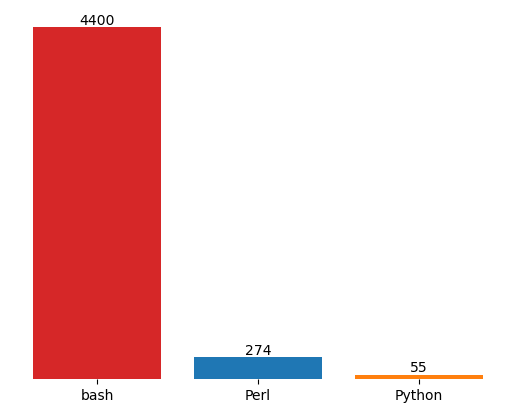
\includegraphics[width=\textwidth]{workflows/SLURM_workflow_solution.png}
	    \end{column}	
	\end{columns}
	\vspace{-12.5em}
	\begin{columns}
		\begin{column}{0.5\textwidth}
			  \pause
			\begin{question}
				How portable is this? How maintainable? How many HPC users are able to accomplish this?\\\pause\hline\vspace{0.5em}
				
				Which conclusions will your users in need of complex analysis steps draw?
			\end{question}	
		\end{column}
		\begin{column}{0.5\textwidth}
			%empty
		\end{column}
	\end{columns}
\end{frame}	

%%%%%%%%%%%%%%%%%%%%%%%%%%%%%%%%%%%%%%%%%%%%%%%%%%%%%%%%%%%%%%%%%%%%%%%%%%%%%%%%
\begin{frame}
  \frametitle{Let them learn! Really?}
  \bcinfo Contemplate \ldots
  \pause
  \begin{question}[When do new users apply for HPC time?]
  	\pause With BIG DATA - or HUGE SIMULATIONS - not for anything else!
  \end{question}
  \pause
  \begin{question}[What do users expect to analyze their data?]
  	\begin{itemize}[<+->]
  		\item all necessary software -- no install hiccups
  		\item to \emph{just} calculate -- no complaints about IO issues or the like
  		\item to get their results \emph{fast} -- after all, it's an HPC system!
  	\end{itemize}
  \end{question}
  \pause
  \begin{question}[What will users think, if their expectations aren't met?]
  	\begin{itemize}[<+->]
  		\item what a workload compared to "my server"??
  		\item what a workload to get here (bureaucracy) and now this??
  		\item abandon HPC!
  	\end{itemize}
  \end{question}	
\end{frame}	feat/admin_talk

%%%%%%%%%%%%%%%%%%%%%%%%%%%%%%%%%%%%%%%%%%%%%%%%%%%%%%%%%%%%%%%%%%%%%%%%%%%%%%%%
\begin{frame}
  \frametitle{Let them learn! Really? - II}
  \begin{question}[How do users plan?]
	\begin{itemize}[<+->]
		\item is data management accounted for?
		\item are their jobs always (well enough) parameterized?
		\item where do get they their infos from? The "internet"? A labmate? A PI?
	\end{itemize}	
  \end{question}
  \pause
  \begin{question}[How do you meet expectations?]
    \begin{itemize}[<+->]
      \item software provisioning schemes
      \item data management support
      \item curated workflows
      \item every item feasible to which extend? With your manpower?
    \end{itemize}
  \end{question}
\end{frame}	


%%%%%%%%%%%%%%%%%%%%%%%%%%%%%%%%%%%%%%%%%%%%%%%%%%%%%%%%%%%%%%%%%%%%%%%%%%%%%%%%
\begin{frame}
	\frametitle{Reproducible Data Analysis}
	\centering
	\begin{onlyenv}<1| handout:0>
		\begin{tikzpicture}
			\path[use as bounding box] (0.7,0) rectangle (12,8);
			\node at (5.5, 5) {\includegraphics[width=0.7\textwidth]{Snakemake/automation.png}};
			\node at (8.5, 2) {\begin{minipage}{0.65\textwidth}
					\textbf{From raw data to final figures:}
					\begin{itemize}
						\item \textbf{document} parameters, tools, versions
						\item \textbf{execute} without manual intervention
					\end{itemize}
				\end{minipage}
			};
		\end{tikzpicture}
	\end{onlyenv}
	\begin{onlyenv}<2| handout:0>
		\begin{tikzpicture}
			\path[use as bounding box] (0.7,0) rectangle (12,8);
			\node at (5.5, 5) {\includegraphics[width=0.7\textwidth]{Snakemake/scalability.png}};
			\node at (8.5, 2) {\begin{minipage}{0.65\textwidth}
					\textbf{Handle parallelization:}
					\begin{itemize}
						\item execute for tens of thousands of datasets
						\item efficiently use any computing platform
					\end{itemize}
				\end{minipage}
			};
		\end{tikzpicture}
	\end{onlyenv}
	\begin{onlyenv}<3| handout:1>
		\begin{tikzpicture}
			\path[use as bounding box] (0.7,0) rectangle (12,8);
			\node at (5.5, 5) {\includegraphics[width=0.7\textwidth]{Snakemake/portability.png}};
			\node at (8.5, 2) {\begin{minipage}{0.65\textwidth}
					\textbf{Handle deployment:}\newline
					be able to easily execute analyses on a different system/platform/infrastructure
				\end{minipage}
			};
		\end{tikzpicture}
	\end{onlyenv}
\end{frame}

%%%%%%%%%%%%%%%%%%%%%%%%%%%%%%%%%%%%%%%%%%%%%%%%%%%%%%%%%%%%%%%%%%%%%%%%%%%%%%%%
\begin{frame}
	\frametitle{Beyond Reproducibility}
	\begin{onlyenv}<1| handout:0>
		\begin{figure}
			\centering
			\includegraphics[width=0.85\textwidth]{Snakemake/reproducibility_only.png}
		\end{figure}
	\end{onlyenv}
	\begin{onlyenv}<2| handout:0>
		\begin{figure}
			\centering
			\includegraphics[width=0.85\textwidth]{Snakemake/reproducibility_empty.png}
		\end{figure}
	\end{onlyenv}
	\begin{onlyenv}<3| handout:0>
		\begin{figure}
			\centering
			\includegraphics[width=0.85\textwidth]{Snakemake/reproducibility_left.png}
		\end{figure}
	\end{onlyenv}
	\begin{onlyenv}<4| handout:1>
		\begin{figure}
			\centering
			\includegraphics[width=0.85\textwidth]{Snakemake/reproducibility_full.png}
		\end{figure}
	\end{onlyenv}
	\footnotesize{\lhref{https://doi.org/10.12688/f1000research.29032.2}{From the official \Snakemake-paper.}}
\end{frame}